\section{Results I: Deterministic Surface Credibility}

\subsection{Model choice}

The deterministic baseline selected Random Forest rather than ridge as the production model. Under leave-one-city-out validation, Random Forest achieved a calibrated RMSE of 115.934 and a calibrated $R^2$ of 0.934, while the ridge comparator performed substantially worse. Under spatial block validation, Random Forest again remained strongest, with a calibrated RMSE of 76.301 and calibrated $R^2$ of 0.980. These statistics are computed against held-out weak targets after city-level rescaling rather than against observed cell-level census labels.

This model split is substantively meaningful. A proxy-population problem based on built form, floor area, transport structure, and service concentration is unlikely to be globally linear, and the stronger Random Forest performance supports the choice of a flexible non-linear baseline without implying truth reconstruction.

Ridge is still valuable in the paper because it shows that the result is not a generic modeling artifact. A simple linear comparator can be beaten by the fixed production configuration, which is consistent with a non-linear urban proxy problem. The point is not that ridge is a bad model in general; the point is that the final City1 baseline should be the model family that most plausibly fits the proxy-allocation task.

\subsection{Grid choice}

The grid benchmark supported 500 m as the fixed operating resolution. The 500 m configuration achieved the best benchmark score (0.248572), outperforming 250 m and 1000 m. The result is interpretable as a detail-stability balance: 250 m is more fragmented and sparse, while 1000 m risks oversmoothing intra-urban differentiation.

That balance is central to the paper. A finer grid can make a proxy surface look more detailed without necessarily making it more informative, while a coarser grid can smooth away the intra-urban structure the paper is trying to represent. The 500 m choice is therefore not a universal optimum; it is the most defensible fixed production compromise for this evidence stack.

\begin{figure}[H]
\centering
\begin{subfigure}[t]{0.48\textwidth}
    \centering
    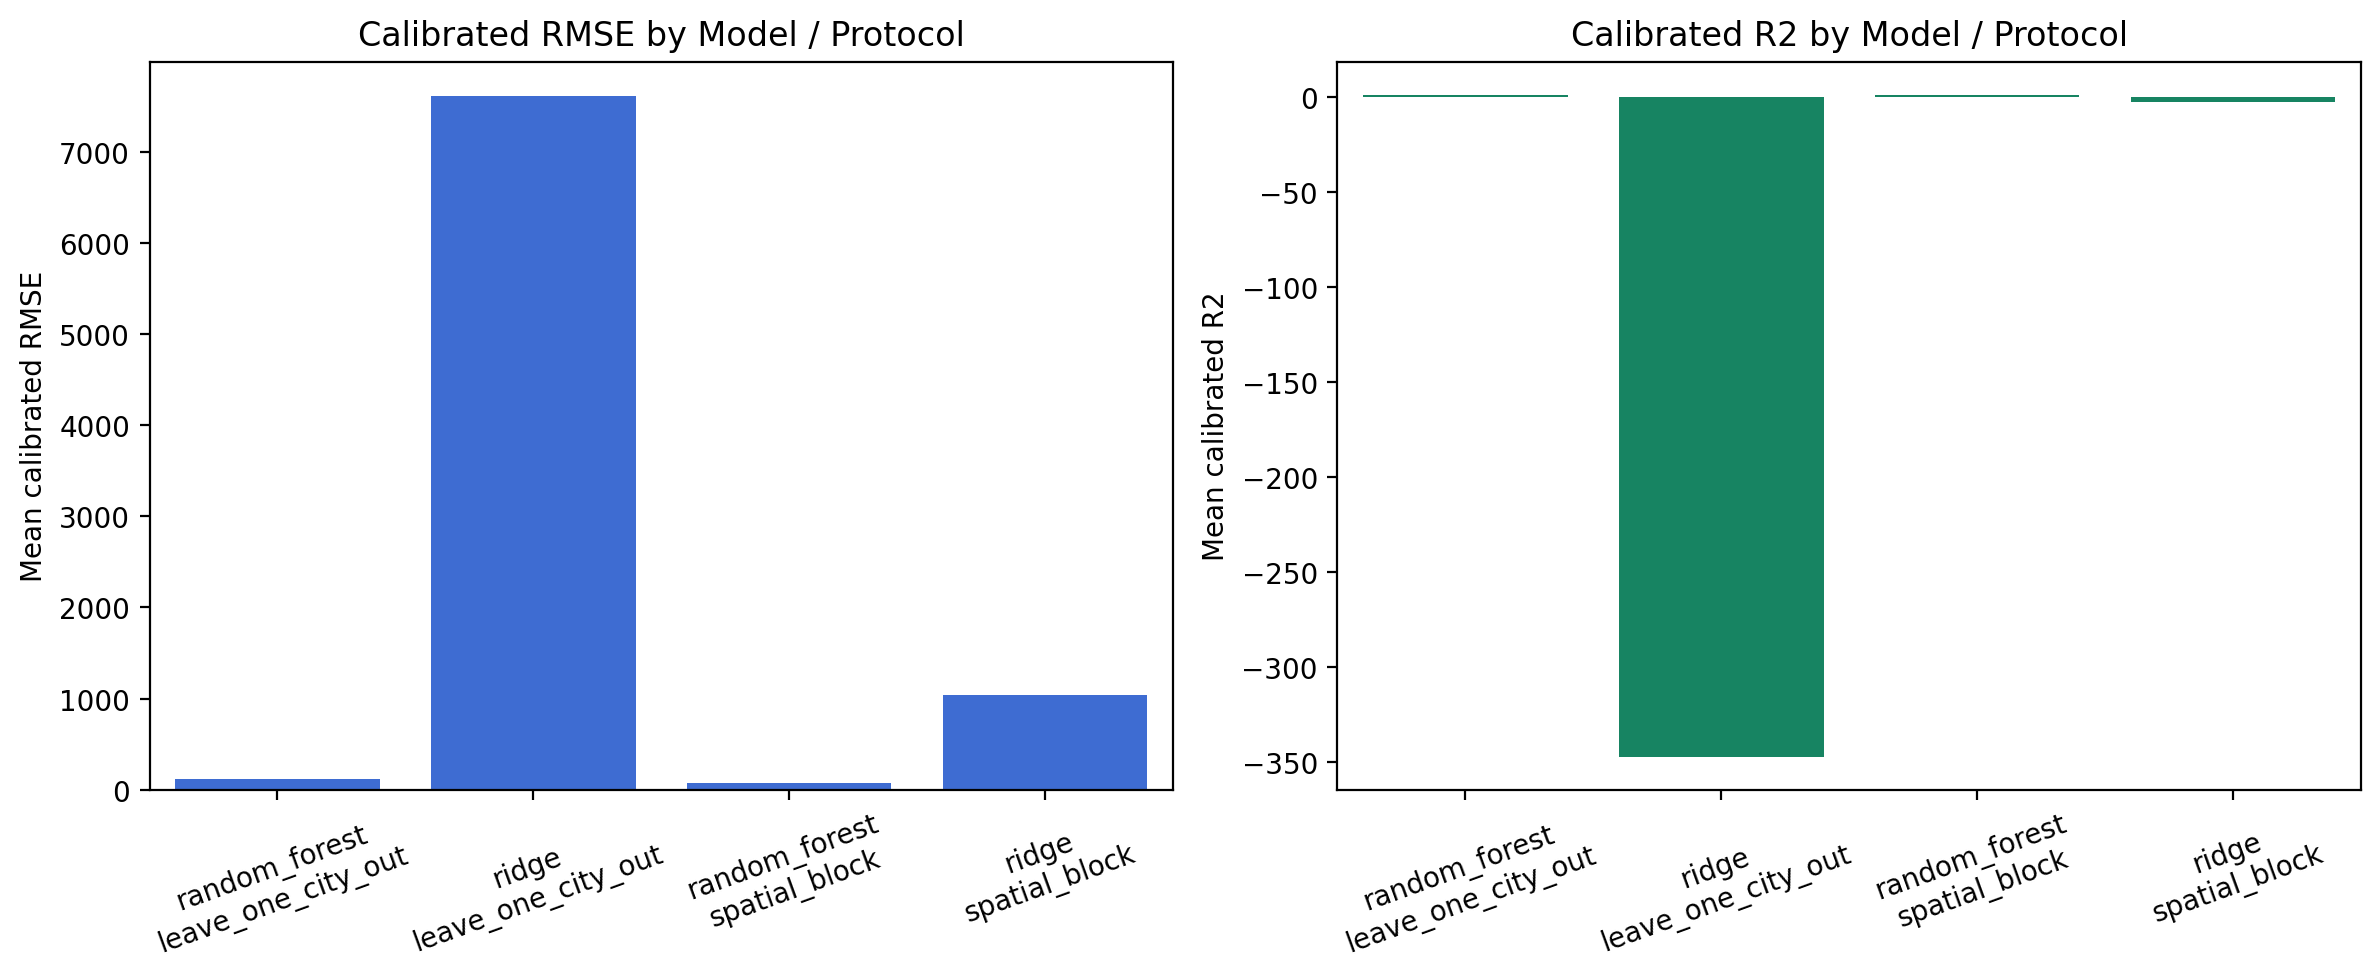
\includegraphics[width=\textwidth]{figures/figure_model_comparison.png}
    \caption{Model comparison}
\end{subfigure}
\hfill
\begin{subfigure}[t]{0.48\textwidth}
    \centering
    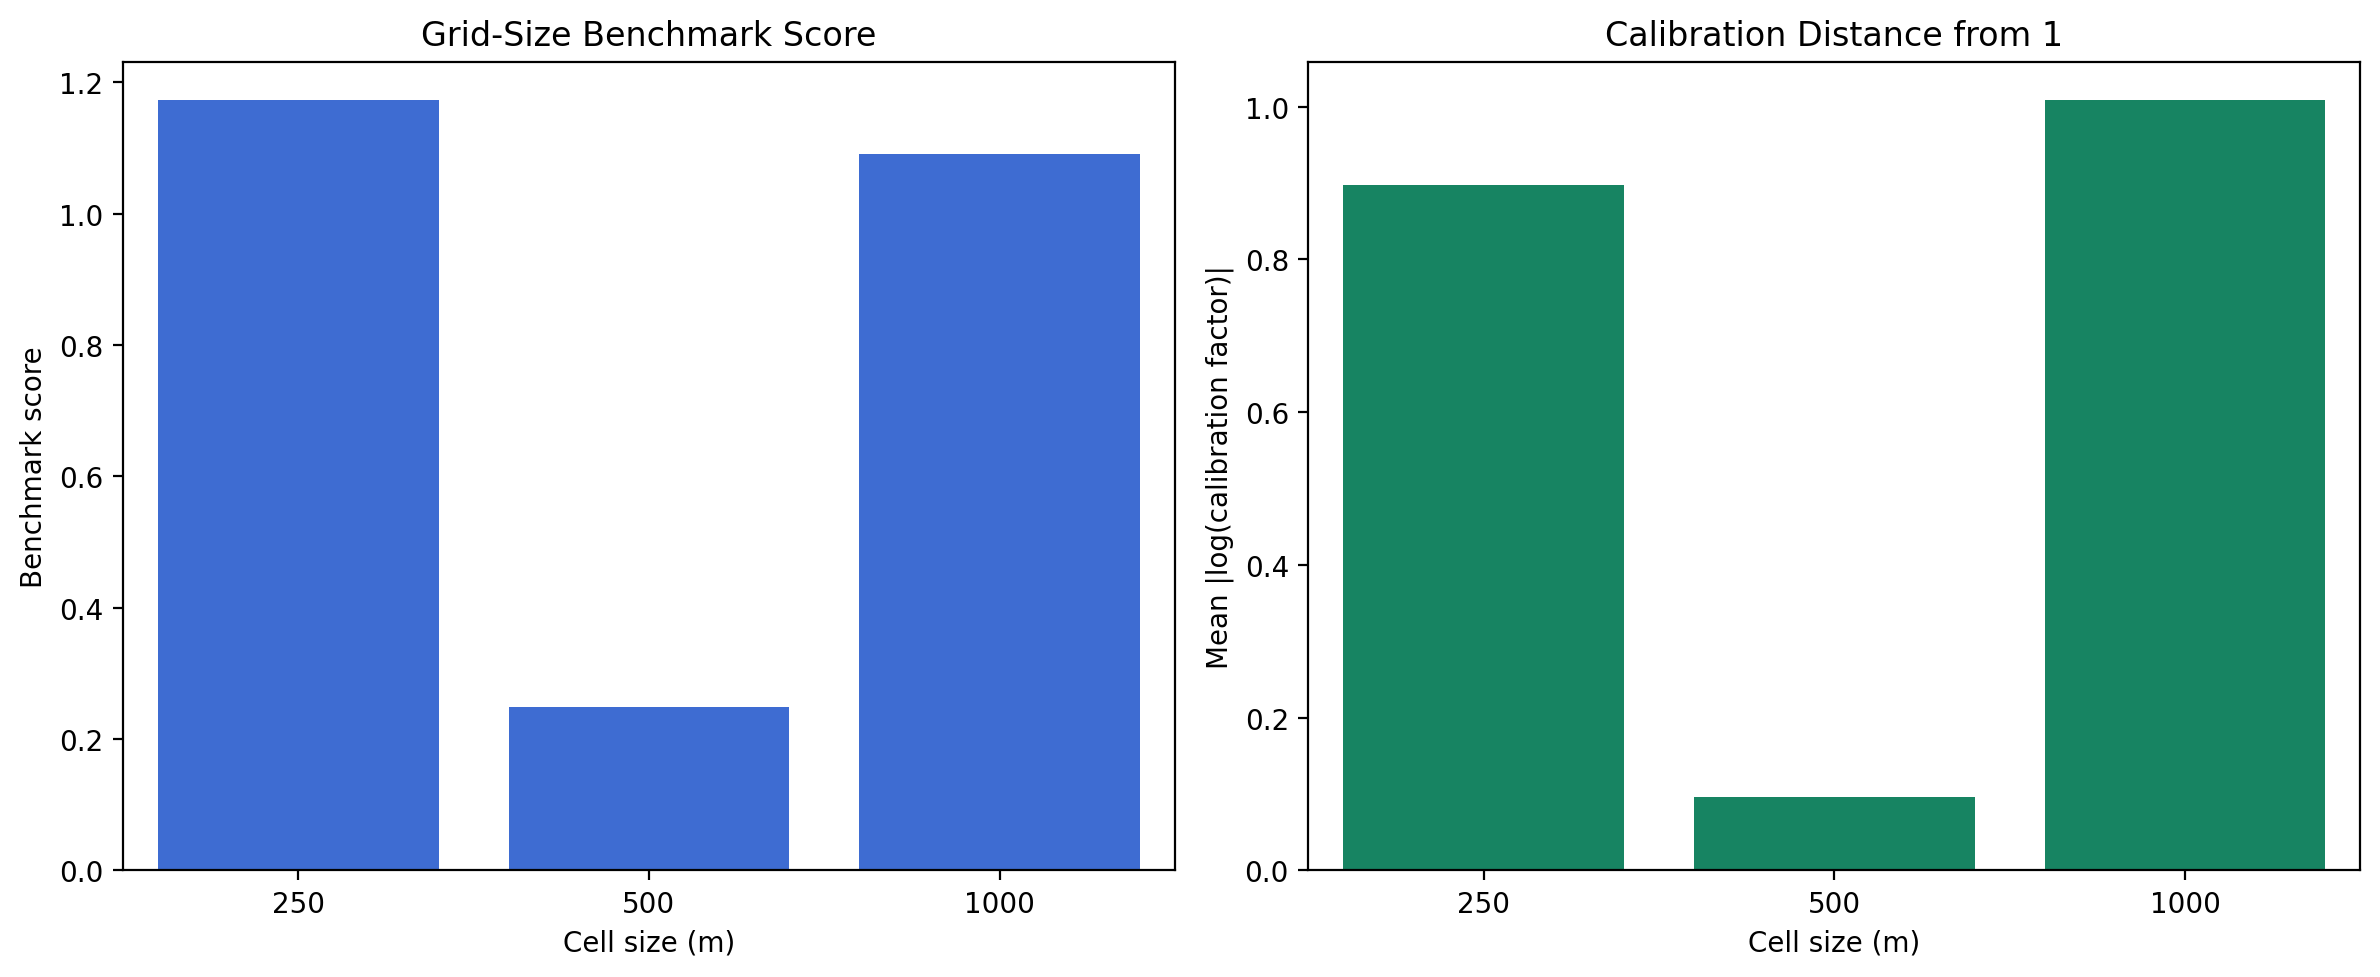
\includegraphics[width=\textwidth]{figures/figure_grid_size_benchmark.png}
    \caption{Grid benchmark}
\end{subfigure}
\caption{Deterministic production selection. Panel (a) shows that Random Forest dominates the ridge comparator under the retained validation protocols. Panel (b) supports 500 m as the fixed production resolution, balancing spatial detail and surface stability.}
\label{fig:deterministic-selection}
\end{figure}

\begin{table}[H]
\centering
\footnotesize
\setlength{\tabcolsep}{4pt}
\renewcommand{\arraystretch}{1.12}
\caption{Core deterministic model and grid validation summary. Calibrated RMSE and calibrated $R^2$ are reported against held-out weak targets after city-level rescaling rather than against observed cell-level census labels.}
\label{tab:core-deterministic-validation}
\begin{adjustbox}{max width=\textwidth}
\begin{tabularx}{\textwidth}{L{1.65cm} Y L{2.10cm} r r r}
\toprule
Component & Setting & Protocol / grid & Calibrated RMSE & Calibrated $R^2$ & Score \\
\midrule
Model & Random Forest & LOCO & 115.934 & 0.934 & -- \\
Model & Ridge & LOCO & 7609.928 & -347.088 & -- \\
Model & Random Forest & spatial block & 76.301 & 0.980 & -- \\
Model & Ridge & spatial block & 1039.817 & -2.690 & -- \\
\midrule
Grid & fixed production choice & 500 m & -- & -- & 0.248572 \\
Grid & finer alternative & 250 m & -- & -- & 1.172821 \\
Grid & coarser alternative & 1000 m & -- & -- & 1.091467 \\
\bottomrule
\end{tabularx}
\end{adjustbox}
\end{table}


\subsection{District benchmark}

District aggregation evidence is strongest in Almaty and weaker in Astana and Shymkent. Almaty reaches Pearson 0.543 and Spearman 0.657 after aggregation, whereas Astana and Shymkent show weak or negative rank-order support. This layer should therefore be interpreted as partial administrative support rather than as truth validation.

The mixed pattern matters because it stops the paper from pretending that district agreement is uniformly strong. Instead, it shows that aggregation can support plausibility where the evidence is good and can remain weak where the support is weaker. That is useful information, but it is not a license to overstate cell-level accuracy.

\begin{figure}[H]
\centering
\begin{subfigure}[t]{0.48\textwidth}
    \centering
    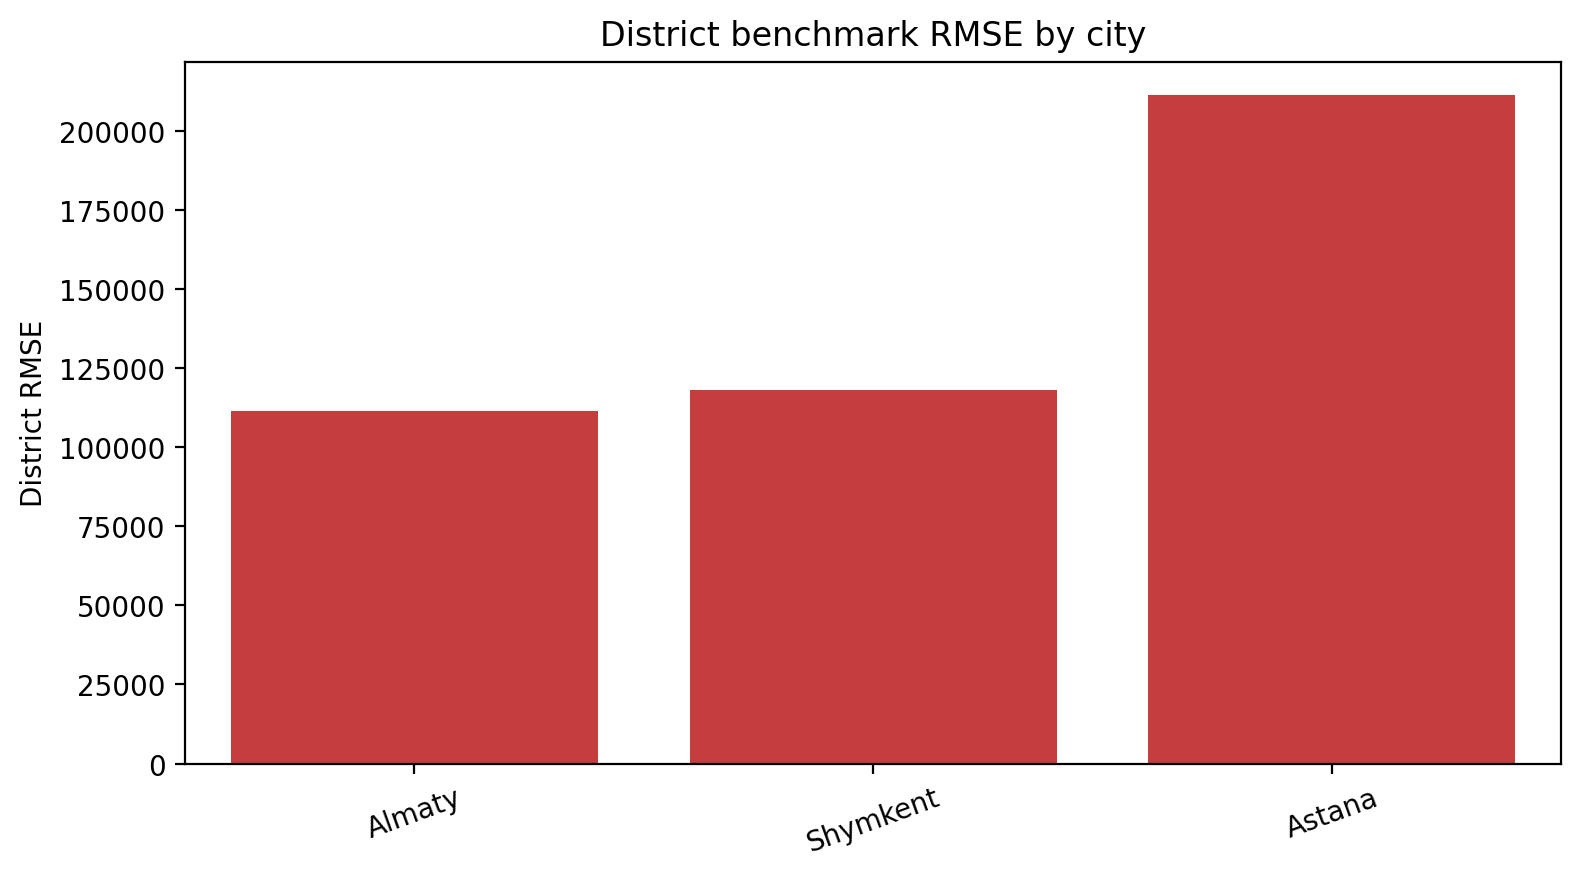
\includegraphics[width=\textwidth]{figures/figure_district_benchmark.png}
    \caption{District benchmark}
\end{subfigure}
\hfill
\begin{subfigure}[t]{0.48\textwidth}
    \centering
    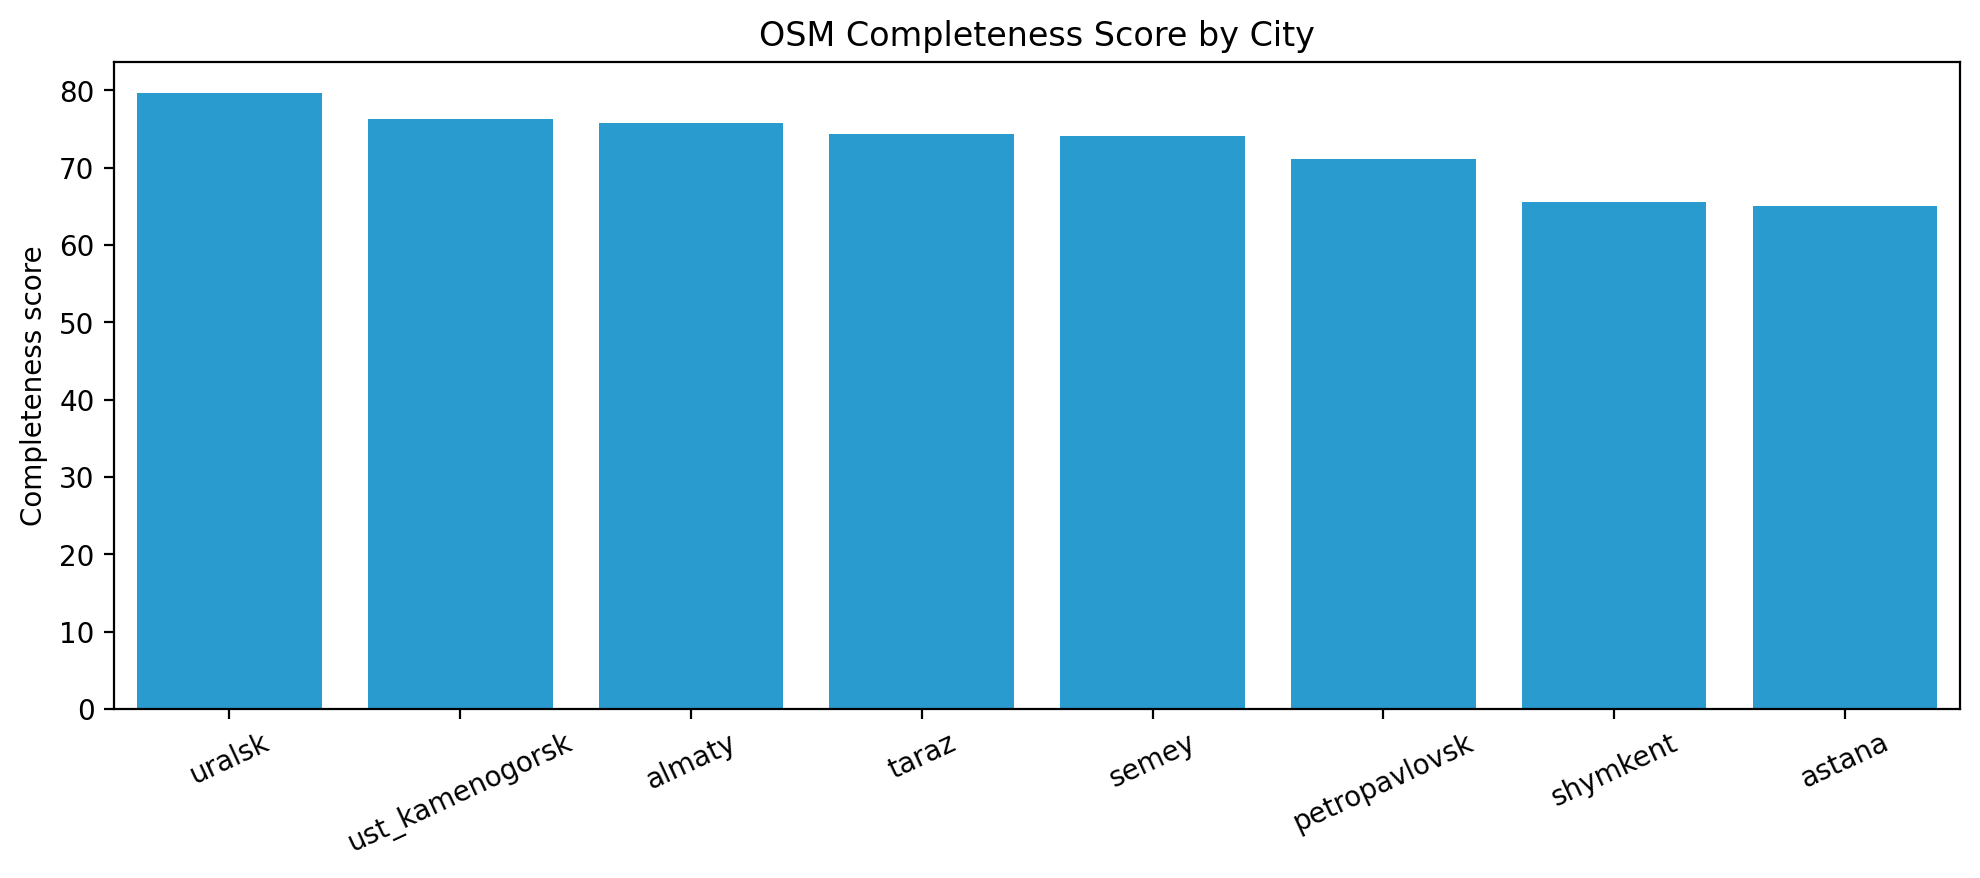
\includegraphics[width=\textwidth]{figures/figure_osm_completeness.png}
    \caption{OSM completeness}
\end{subfigure}
\caption{Internal and support-context evidence for the deterministic baseline. Panel (a) reports district aggregation comparison where administrative references were available. Panel (b) reports OSM completeness, which is used as interpretation context rather than as a direct accuracy metric.}
\label{fig:district-osm}
\end{figure}

\begin{table}[H]
\centering
\caption{Deterministic district benchmark summary. This layer is interpreted as partial administrative support after aggregation rather than as cell-level truth validation.}
\label{tab:district-benchmark-unified}
\begin{tabular}{lrrrrr}
\toprule
City & Compared districts & RMSE & MAPE & Pearson $r$ & Spearman $r$ \\
\midrule
Almaty & 6 & 111379.724 & 37.691 & 0.543 & 0.657 \\
Astana & 5 & 211191.733 & 83.186 & -0.277 & -0.300 \\
Shymkent & 3 & 118069.168 & 42.698 & -0.169 & -0.500 \\
\bottomrule
\end{tabular}
\end{table}



\subsection{External benchmark}

External structural comparison shows complementary support rather than a single winner. WorldPop is strongest for broad correlation, with Pearson 0.877. GHS-POP is strongest for hotspot-sensitive structure, with Spearman 0.834, top-decile overlap 0.614, and hotspot IoU 0.443. This is scientifically useful because it shows that different independent products align with different aspects of the inferred surface.

The interpretation is therefore comparative, not adjudicative. WorldPop helps show whether the surface behaves similarly at a broad spatial level. GHS-POP helps show whether hotspot structure is in the right general place. Neither result means the City1 surface has been validated against truth.

\begin{figure}[H]
\centering
\begin{subfigure}[t]{0.48\textwidth}
    \centering
    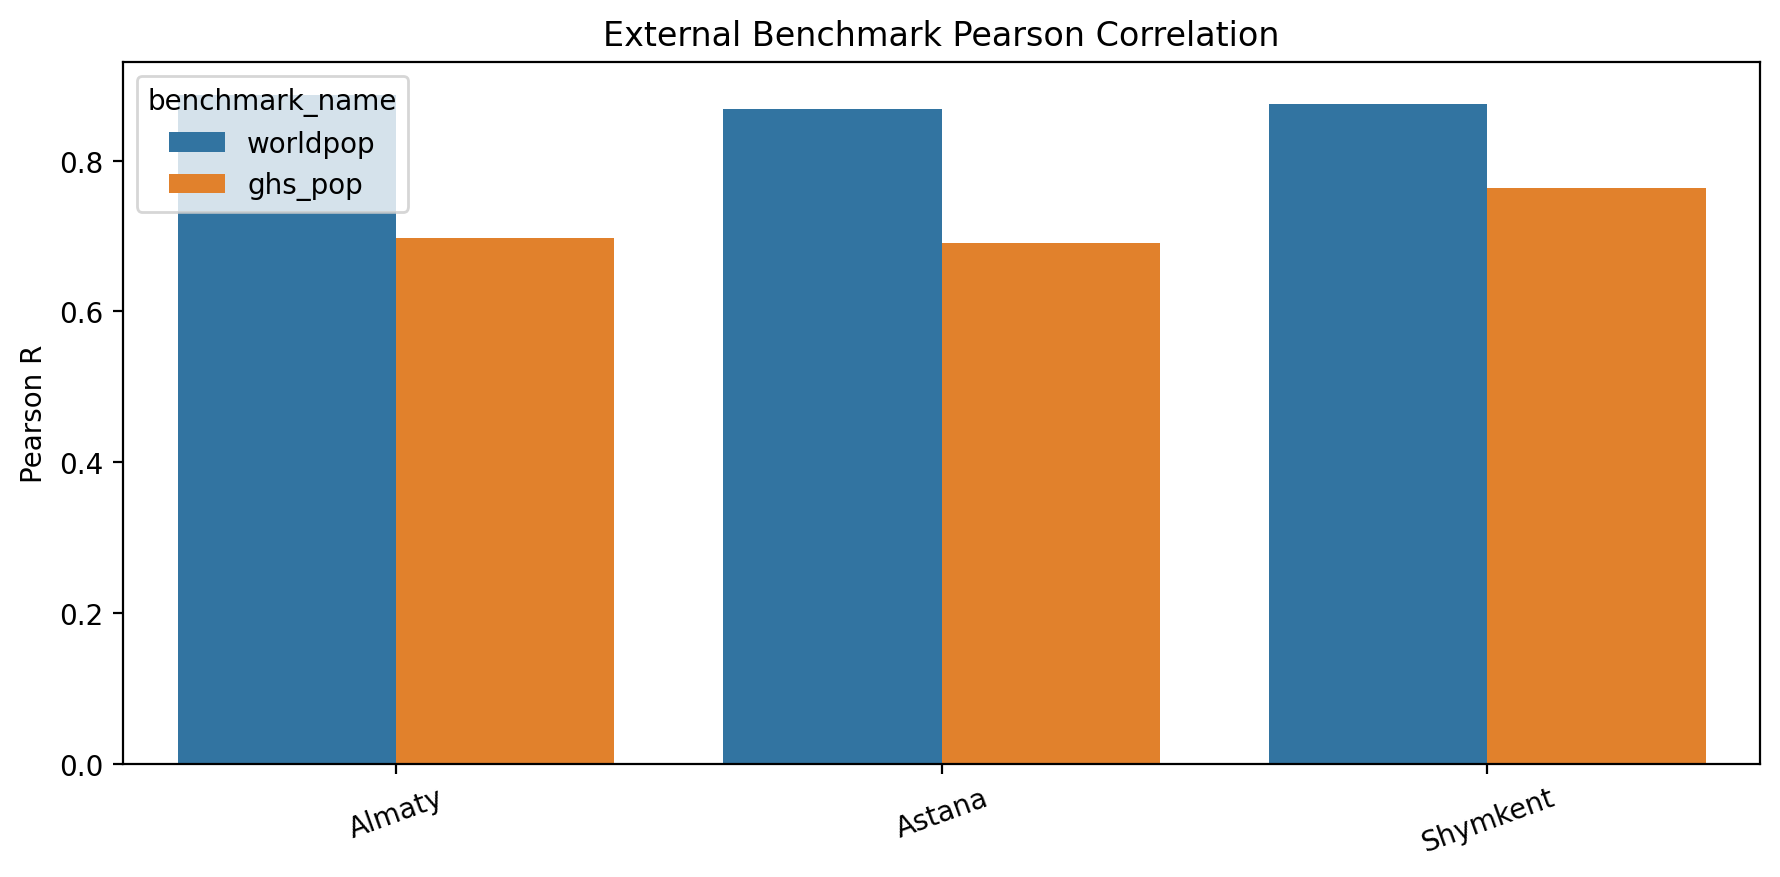
\includegraphics[width=\textwidth]{figures/figure_external_benchmark_pearson.png}
    \caption{Overall correlation}
\end{subfigure}
\hfill
\begin{subfigure}[t]{0.48\textwidth}
    \centering
    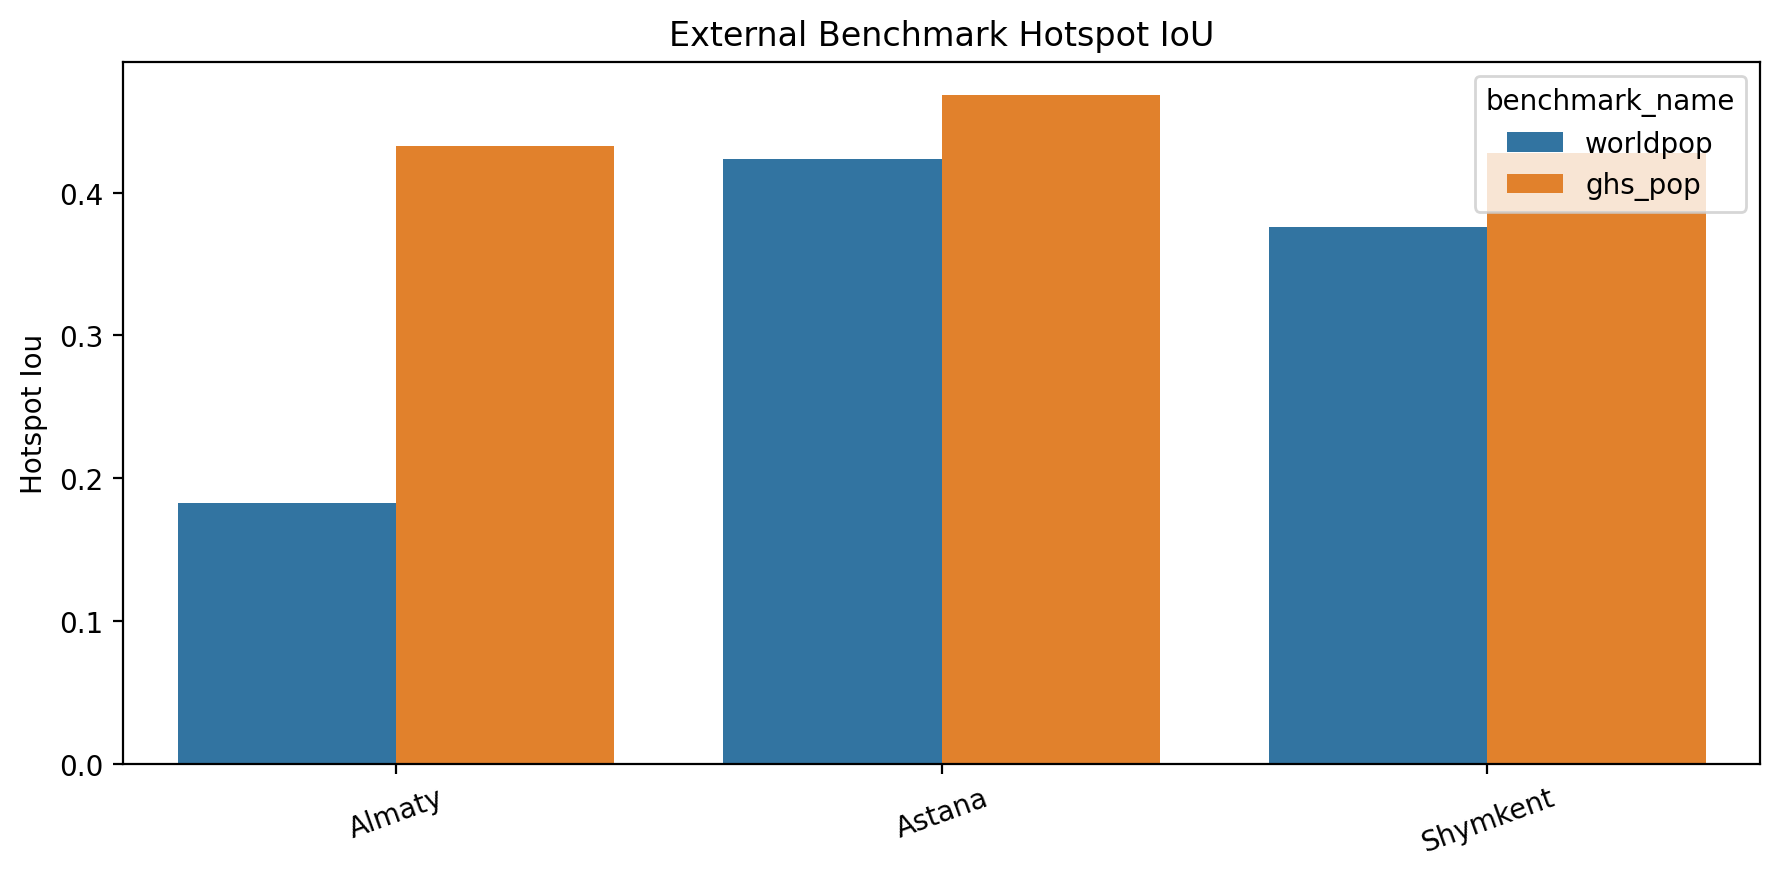
\includegraphics[width=\textwidth]{figures/figure_external_benchmark_hotspot_iou.png}
    \caption{Hotspot-sensitive agreement}
\end{subfigure}
\caption{External structural comparison for the deterministic baseline. WorldPop supports broad structural correlation more strongly, while GHS-POP supports hotspot-sensitive agreement more strongly. These are structural comparators rather than ground truth.}
\label{fig:external-structure}
\end{figure}

\begin{table}[H]
\centering
\caption{Deterministic external benchmark summary from independent gridded population products. These comparisons are used as structural agreement checks rather than as direct truth validation.}
\label{tab:external-benchmark-unified}
\begin{tabular}{lrrrr}
\toprule
Benchmark & Pearson $r$ & Spearman $r$ & Top-decile overlap & Hotspot IoU \\
\midrule
WorldPop & 0.877 & 0.831 & 0.483 & 0.327 \\
GHS-POP & 0.718 & 0.834 & 0.614 & 0.443 \\
\bottomrule
\end{tabular}
\end{table}



\subsection{Ablation}

The full feature set remains strongest overall, while built-form-only is the strongest reduced predictor family. The full feature configuration achieves a calibrated RMSE of 115.934 and calibrated $R^2$ of 0.934. Built-form-only remains close behind at calibrated RMSE 120.656 and calibrated $R^2$ 0.929, while transport-only and POI/services-only are much weaker. Calibration also materially improves the final output, with a full-model RMSE gain of 135.821 between raw and calibrated outputs.

The ablation story is important because it reveals the core signal family without reducing the paper to a single feature-engineering trick. Built form carries the dominant reduced-family signal, which is intuitive for urban population allocation, but the full stack remains strongest because the city surface is shaped by multiple types of open-data evidence at once. That combination is what makes the calibrated proxy surface more credible than any one family alone.

\input{tables_tex/table6_ablation_summary.tex}

\subsection{Qualitative plausibility}

Qualitative plausibility is locked to Almaty and Astana. In both cities, dense residential and central mixed-use zones tend to receive higher predicted population, while peripheral open or weak-built zones tend to remain low. Almaty provides the stronger completeness case and therefore the stronger visual plausibility reading. Astana remains more cautious but still preserves interpretable urban morphology. This layer supports plausibility, not cell-level truth.

The qualitative reading is intentionally modest. It does not say the map is “correct”; it says the map is consistent with visible urban structure in a way that supports the bounded proxy claim. That is exactly the kind of evidence a reviewer expects when the paper cannot rely on true cell-level census labels.

\begin{figure}[H]
\centering
\begin{subfigure}[t]{0.49\textwidth}
    \centering
    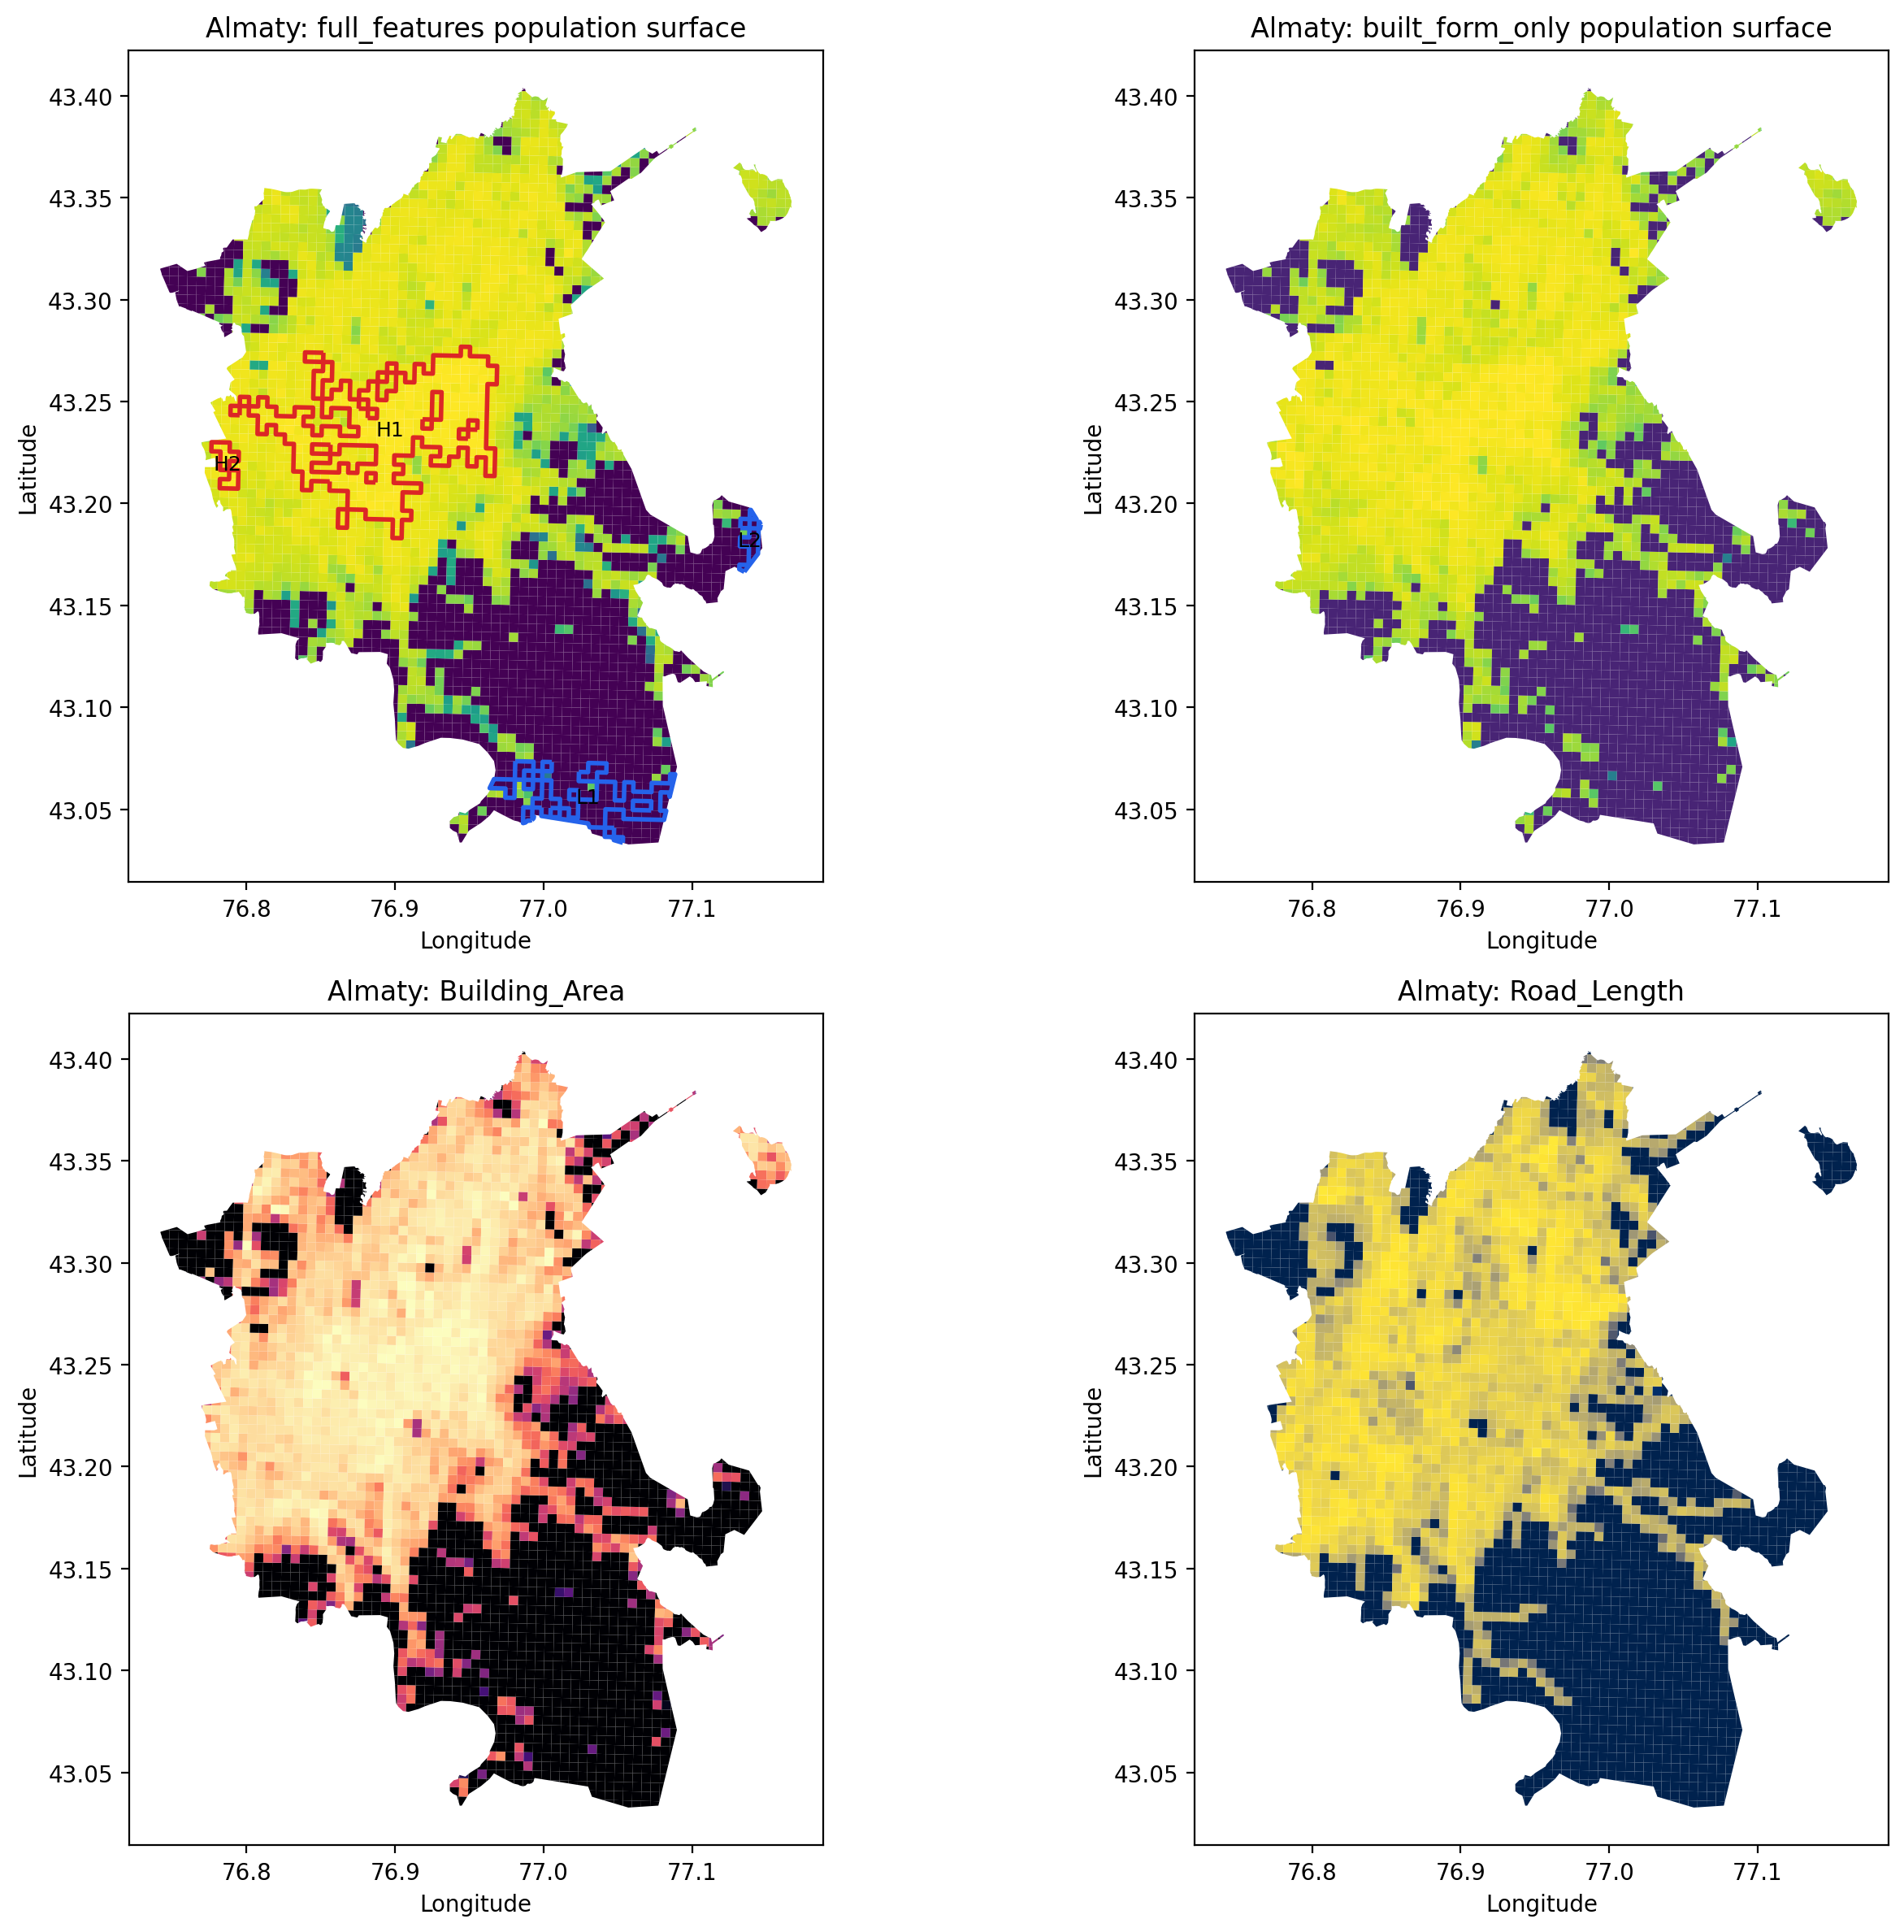
\includegraphics[width=\textwidth]{figures/figure_qualitative_overview_almaty.png}
    \caption{Almaty overview}
\end{subfigure}
\hfill
\begin{subfigure}[t]{0.49\textwidth}
    \centering
    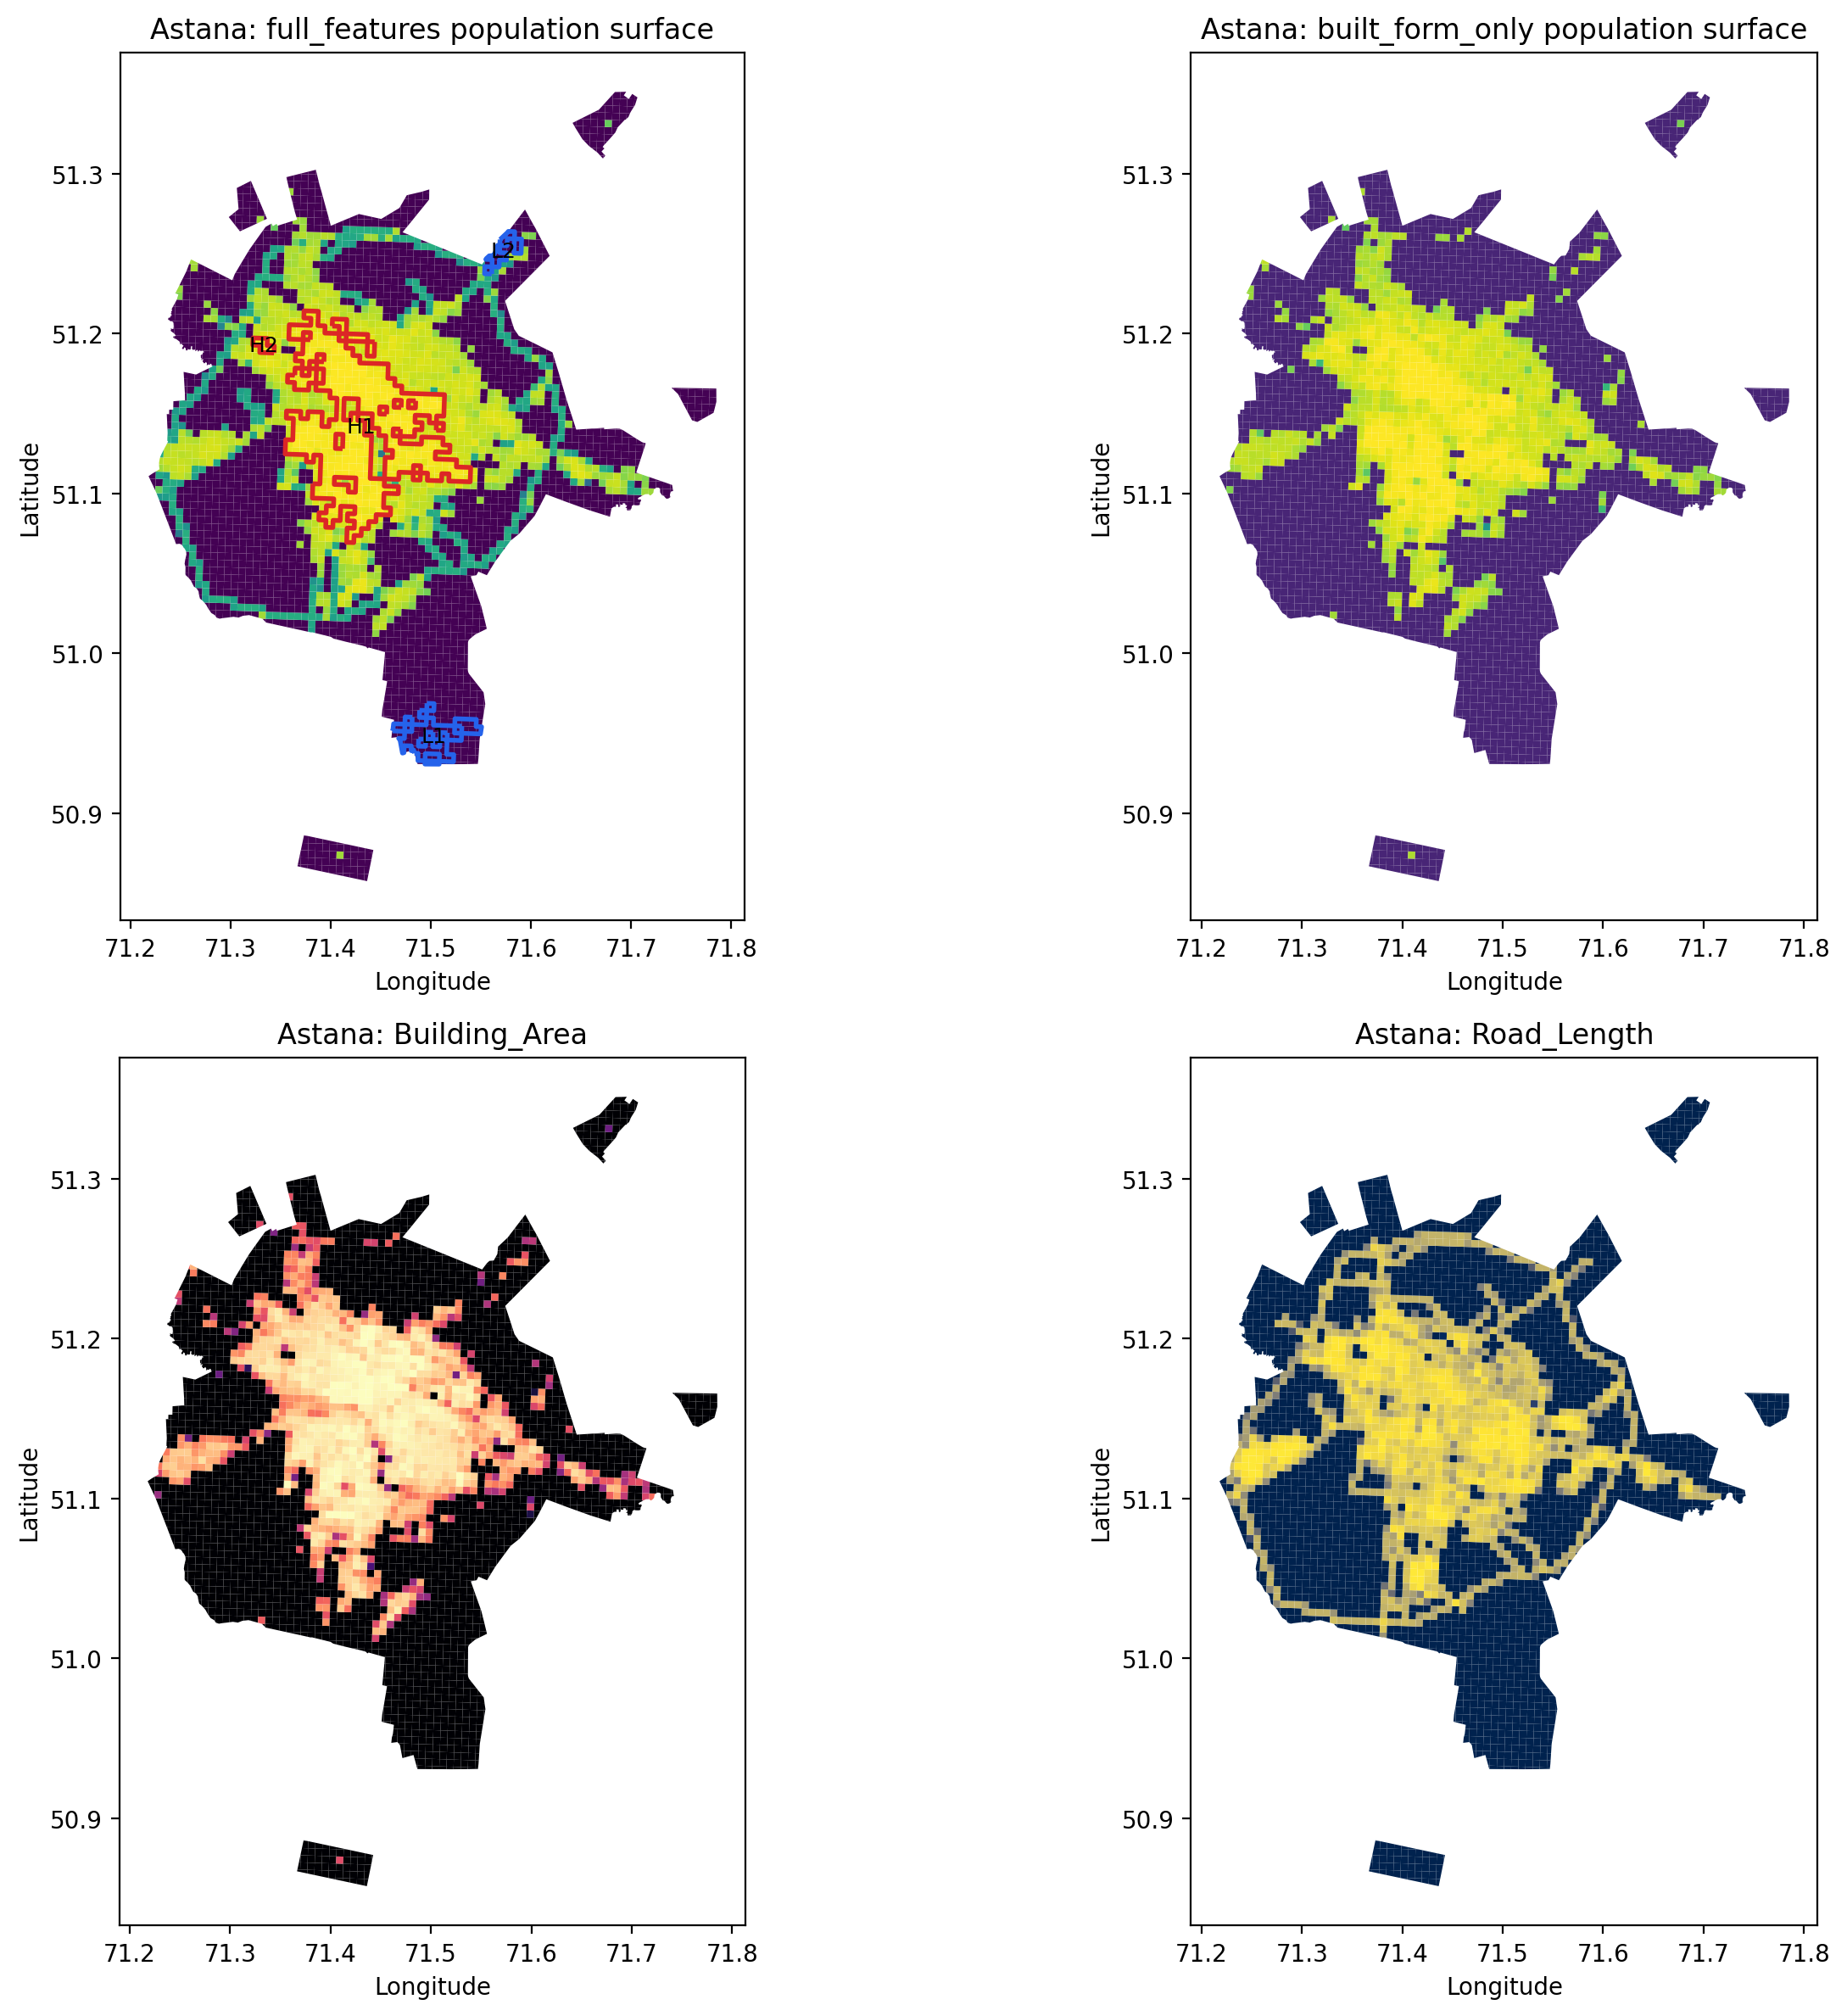
\includegraphics[width=\textwidth]{figures/figure_qualitative_overview_astana.png}
    \caption{Astana overview}
\end{subfigure}
\caption{Qualitative plausibility overview for the deterministic baseline. The maps compare the calibrated proxy surface with visible built-environment structure and are interpreted as urban-structural plausibility evidence rather than as truth validation.}
\label{fig:qualitative-overview-unified}
\end{figure}
